%======================
% Step 0
%======================
\begin{figure}[ht]
  \centering
  \begin{minipage}[c]{\textwidth}
    \begin{lstlisting}[escapeinside={<@}{@>},aboveskip=0.1em,belowskip=0.1em]
    let x = if flip() <@\textcolor{purple}{then}@> uniform(0,2) <@\textcolor{purple}{else}@> gaussian(0,1) in
    let y = if 1.5 <@\textcolor{red}{>}@> x <@\textcolor{purple}{then}@> 1.8 <@\textcolor{purple}{else}@> 0.3 in x <@\textcolor{orange}{<=}@> y
    \end{lstlisting}      
  \end{minipage}
        
  \vspace{0.8em}

  \begin{minipage}[c]{\textwidth}
  \centering
  \scalebox{0.58}{
  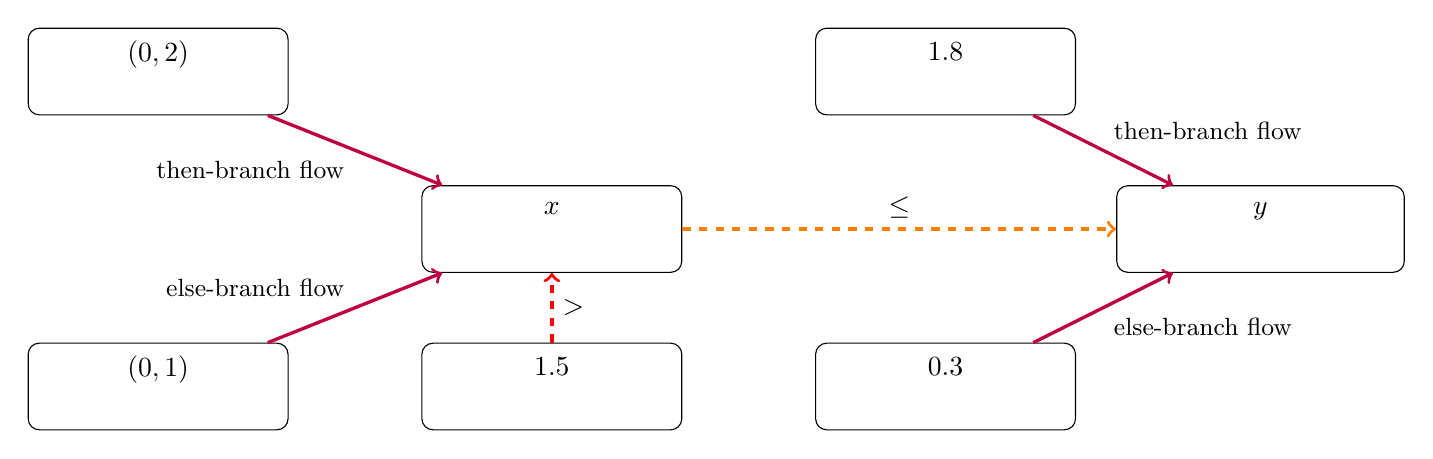
\begin{tikzpicture}[
      floatnode/.style={draw, rounded corners, minimum width=3.3cm, minimum height=1.1cm, align=center},
      flow/.style={->, very thick, draw=purple},
      constraintgt/.style={->, very thick, dashed, draw=red},
      constraintleq/.style={->, very thick, dashed, draw=orange}
  ]

  % ==== FLOAT NODES ====

  \node[floatnode] (u) at (-6, 2) {
      $\uniform(0,2)$ \\
      \phantom{$\floattype{\{\cleq{0.3}, \clt{1.5}, \cleq{1.8}\}}{\top}$}
  };

  \node[floatnode] (g) at (-6, -2) {
      $\gaussian(0,1)$ \\
      \phantom{$\floattype{\{\cleq{0.3}, \clt{1.5}, \cleq{1.8}\}}{\top}$}
  };

  \node[floatnode] (x) at (-1, 0) {
      $x$ \\
      \phantom{$\floattype{\{\cleq{0.3}, \clt{1.5}, \cleq{1.8}\}}{\top}$}
  };

  \node[floatnode] (c15) at (-1, -2) {
      1.5 \\
      \phantom{$\floattype{\{\cleq{0.3}, \clt{1.5}, \cleq{1.8}\}}{\{1.5\}}$}
  };

  \node[floatnode] (y) at (8, 0) {
      $y$ \\
      \phantom{$\floattype{\{\cleq{0.3}, \clt{1.5}, \cleq{1.8}\}}{\{0.3,1.8\}}$}
  };

  \node[floatnode] (c18) at (4.0, 2) {
      1.8 \\
      \phantom{$\floattype{\{\cleq{0.3}, \clt{1.5}, \cleq{1.8}\}}{\{1.8\}}$}
  };

  \node[floatnode] (c03) at (4.0, -2) {
      0.3 \\
      \phantom{$\floattype{\{\cleq{0.3}, \clt{1.5}, \cleq{1.8}\}}{\{0.3\}}$}
  };

  % ==== DATA FLOW EDGES ====

  \draw[flow] (u) -- node[below left] {\small then-branch flow} (x);
  \draw[flow] (g) -- node[above left] {\small else-branch flow} (x);

  \draw[flow] (c18) -- node[above right] {\small then-branch flow} (y);
  \draw[flow] (c03) -- node[below right] {\small else-branch flow} (y);

  % ==== COMPARISON EDGES ====

  \draw[constraintgt] (c15) -- node[right] {$>$} (x);
  \draw[constraintleq] (x) -- node[above] {$\leq$} (y);

  \end{tikzpicture}
  }
  \end{minipage}
\caption{Constraint graph for float types. Solid arrows represent data flow, and dashed arrows constraints.}
\label{fig:constraint-graph-gaussian}
\end{figure}
